% !TeX root = main_long.tex
\section{RQ1: Coverage of the VCF specification}
\subsection{Method}
\label{sec:m-rq1}
We assess correspondence between VCF specification and VCF Core in both directions: from specification requirements to the vocabulary representation, and from the vocabulary to a curated inventory of VCF constructs.

\subsection{VCF specification to VCF Core Representation}
The first assessment starts from pinned, digest-verified VCF 4.1--4.5 specification \LaTeX{} files.
Scripts read these files, extract the explicit reserved INFO and FORMAT declarations, and record a decision for every section so that no passage is skipped (\href{https://github.com/ecrum19/SWAT4HCLS_2027/tree/main/RQ1/methodology/scripts}{\path{RQ1/methodology/scripts/}}).
\emph{Requirements} are not extracted automatically, but were drafted from the text with AI assistance~\cite{anthropic2026claudeopus5,openai2026gpt6astra}, linked to their source passages, and reviewed by the first author (\href{https://github.com/ecrum19/SWAT4HCLS_2027/blob/main/RQ1/methodology/inputs/requirements.json}{\path{requirements.json}}; procedure in \href{https://github.com/ecrum19/SWAT4HCLS_2027/blob/main/RQ1/EXPERIMENT.md}{\path{RQ1/EXPERIMENT.md}}).
A \emph{requirement} states a specification rule as a question with a checkable answer, following established competency-question and requirements-specification practices~\cite{gruninger1995methodology,suarezfigueroa2009orsd,lot2022}.
For example, R27 asks: ``Can local allele indices map to global record alleles?'', the rule Listing~\ref{lst:vcf-example} illustrates.
Binary encoding, compression, indexing, producer estimation algorithms, and general invalid-input rejection are outside the scope of this assessment.

\paragraph{Cases and expected answers.}
A \emph{case} pairs one requirement and VCF version with a \emph{fixture}: a small VCF file constructed to expose the corresponding specification rule. 
The fixture is materialized as a \emph{witness} graph using VCF Core and queried with SPARQL~\cite{sparql2013}.
Each case also has an \emph{expected answer}, derived from the specification and fixture before the query is executed, adapting SAMOD and executable ontology-testing approaches~\cite{samod2016,blomqvist2012ontologytesting,wisniewski2019competencyquestions}. 
Where possible, fixtures and expected values are taken directly from examples in the VCF specification.

The query is evidence of coverage, not the source of the expected result. 
Each case passes only if the RDF graph contains enough information to reproduce an answer defined independently from the specification and fixture. 
Tailoring a query to the vocabulary cannot recover information that is absent from the graph.

Answers are compared as multisets of string-valued rows: missing, extra, or duplicated rows fail, while requirements concerning order explicitly project the relevant ordinal. 
Values such as \texttt{30} and \texttt{30.0} therefore remain distinct. 
The fixture's declared VCF version must also match the version assigned to the case.

\paragraph{Worked cases.}
Listing~\ref{lst:vcf-example} illustrates the rules that requirements R27 and R21 test, in place of the registered fixtures.
R27 concerns the local-allele mapping that Figure~\ref{fig:model} follows for \texttt{S1} on line 8, where depth 30 belongs to ALT allele 2, \texttt{C}.
In \texttt{S2}, \texttt{LAA=1} selects \texttt{A} instead, so the depth 9 at the same local position belongs to ALT allele 1.
Listing~\ref{lst:rq1-example} retrieves that mapping; restricted to line 8, it expects the rows \mbox{\texttt{(1, S1, 0, 0, G, 20)}}, \mbox{\texttt{(1, S1, 1, 2, C, 30)}}, \mbox{\texttt{(1, S2, 0, 0, G, 12)}}, and \mbox{\texttt{(1, S2, 1, 1, A, 9)}} for record position, sample, local index, global index, allele, and depth.
A representation that dropped \texttt{LAA} would attach both second depths to ALT allele 1 and fail the case.

\begin{lstlisting}[float=htbp,caption={A query retrieving the local-to-global allele mapping that R27 tests.},label={lst:rq1-example}]
PREFIX vcfc: <https://w3id.org/vcf-core/vocab#>
SELECT ?pos ?sample ?index ?global ?allele ?depth WHERE {
  ?record vcfc:pos ?pos ; vcfc:hasCall/vcfc:hasSampleCall ?call .
  ?call vcfc:sampleId ?sample ; vcfc:hasFormatValue ?field .
  ?field vcfc:declaredBy/vcfc:fieldId "LAD" ; vcfc:hasValueItem ?item .
  ?item vcfc:valueIndex ?index ; vcfc:itemValue ?depth ; vcfc:forAllele ?a .
  ?a vcfc:alleleIndex ?global ; vcfc:alleleValue ?allele .
} ORDER BY ?pos ?sample ?index
\end{lstlisting}

R21 concerns missingness, which line 10 of Listing~\ref{lst:vcf-example} exhibits.
\texttt{S1} contains \texttt{./.:.:.} which explicitly reports a missing \texttt{LAD}. 
\texttt{S2} contains \texttt{0/0} which drops the trailing \texttt{LAA} and \texttt{LAD} subfields altogether.
The two remain distinguishable, so the expected results for line 10 are \texttt{(S1, ".")} and \texttt{(S2, unbound)}.
The expanded query follows each sample's \texttt{LAD} field, using \term{OPTIONAL} to retain a row when that field is absent.
The cases for both requirements above use their own fixtures, queries, and expected results, and are documented in \href{https://github.com/ecrum19/SWAT4HCLS_2027/tree/main/RQ1/methodology}{\path{RQ1/methodology/}} in the experimental repository.

\paragraph{Retrieval, controls, and scoring.}
Each case runs in both sample profiles on two \emph{axes}.
\emph{Preservation} permits decoding values from literals, whereas \emph{structure} requires graph relationships and prohibits the string-decomposition functions \term{REPLACE}, \term{SUBSTR}, \term{STRBEFORE}, and \term{STRAFTER}.
An empty-graph control rejects queries that return the expected answer without data.
A predicate-deletion control requires the answer to change after deleting at least one referenced property; it establishes dependence on some vocabulary data, rather than on every property mentioned.
Requirements are scored per applicable version, profile, and axis as demonstrated when all cases pass, partial when some pass, not demonstrated when all fail, and unassessed when no case exists.
Only demonstrated requirements enter the numerator of coverage; all applicable requirements, including unassessed ones, remain in the denominator with equal weight.

The VCF Core vocabulary repository's \href{https://github.com/ecrum19/vcf-core-vocabulary/blob/main/scripts/vcf_examples.py}{Python materializer}\footnote{\url{https://github.com/ecrum19/vcf-core-vocabulary/blob/main/scripts/vcf_examples.py}} builds witnesses from fixtures.
The materializer, vocabulary, and queries share an author, so a common misunderstanding remains possible despite separately authored answers and controls: the controls establish dependence on graph data, not that a question or expected answer correctly interprets the specification.
Test selection also favours rules with defensible examples.
RQ2 tests whether the same questions expose representation differences in a separate implementation, but does not provide independent validation of the questions.
Separately, reserved INFO/FORMAT Number/Type declarations are extracted from the specification texts and compared with the corresponding version registries.
This tests explicit declarations, independently of prose interpretation.

\subsection{Curated inventory}
The second assessment links 104 VCF 4.5 logical constructs to vocabulary terms and supporting evidence.
The inventory classifies whether information is preserved, structurally retrievable, and enforced by a validation rule.
Representation is full when both preservation and structure are supported, partial when only preservation is supported, and absent otherwise.
Enforcement is recorded separately and does not contribute to the representation score.
The two assessments count different things and are not combined: the first inspects specification-derived requirements in both profiles, whereas the inventory records curated judgments about VCF constructs in expanded profile only.

\subsection{Results}
\label{sec:evidence}

\paragraph{Declarations and assessment corpus.}
All \textbf{333} explicit reserved Number/Type declarations extracted from VCF 4.1--4.5 match the version registries, with no missing or differing row.
VCF 4.5's registry contains 122 reserved definitions: 51 INFO and 71 FORMAT, including three parameterized base-modification families.
These are different populations: the comparison includes only explicit, comparable declarations, while older specifications also define reserved keys in prose without complete Number/Type information.
Agreement is therefore weighted towards VCF 4.3--4.5 and does not settle declaration--prose inconsistencies, such as CNL/CNP declaring \texttt{Number=G} while describing copy-number ordering.

The VCF specification was fragmented into \textbf{94 requirements}, \textbf{38 fixtures}, \textbf{210 cases}, and \textbf{79 distinct queries}, linked to specification passages and expected answers.
Nine fixtures reproduce published specification examples exactly; the others are minimal files instantiating stated rules.
Interpretation statements also vary in specificity: 56 are requirement-specific, 29 generic, and nine explicitly unassessed.
During our review we identified inconsistent specification examples, including three issues (such as \href{https://github.com/samtools/hts-specs/issues/869}{hts-specs\#869}\footnote{\url{https://github.com/samtools/hts-specs/issues/869}}) reported to the maintainers and one previously reported issue, documented in the experimental repository.
Where an interpretation could be established, affected requirements were scored; unresolved cases remained unassessed and counted against coverage.

\paragraph{Executed coverage.}
The 210 cases exercise \textbf{53 of 94 requirements} in at least one applicable version.
All 210 preservation tests passed in each profile, as did all 210 expanded-structure tests.
Condensed structure passed 165 and failed 45 tests, all concerning sample-level FORMAT access held in vectors rather than individual resources.
Every passing case rejected the empty-graph control and changed its answer under at least one referenced-predicate deletion.
The worked cases follow this pattern: R27 and R21 both pass preservation in both profiles, and structure only in the expanded profile.
Figure~\ref{fig:requirement-results} aggregates these outcomes by requirement and applicable version; an untested requirement remains in the denominator.

\begin{figure}[htbp]
\centering
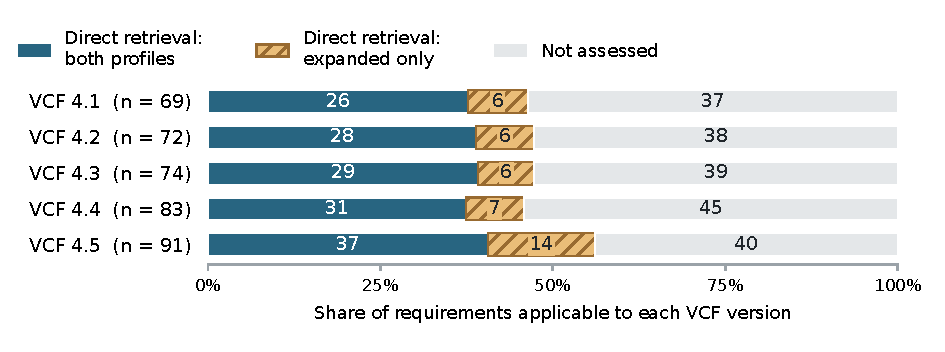
\includegraphics[width=\linewidth]{figures/requirement-coverage.pdf}
\caption{
  Coverage of registered requirements by VCF version; the legend names the three categories. 
  Colored segments pass preservation in both profiles. 
  Widths show percentages of applicable requirements and labels provide counts. 
  Requirements may apply to more than one version.
  }
\label{fig:requirement-results}
\end{figure}

For VCF 4.5, 51 of 91 requirements (56.0\%) have demonstrated preservation in both profiles; 37 also support direct retrieval in condensed data, while 40 remain unassessed.
Of the 40 unassessed requirements, 37 await fixtures and queries, one requires further interpretation, and two require coverage of all reserved INFO and FORMAT keys.
Most missing coverage therefore reflects absent tests rather than failures: the tested structural failures concern only the condensed representation, and their expanded counterparts pass.

\paragraph{Curated inventory.}
All \textbf{104} inventoried VCF 4.5 logical constructs were classified as preserved and structured.
\textbf{87} of these constructs have a validation rule (i.e. a SHACL shape or a decoded check) testing a stated requirement; the inventory and its evidence are in \href{https://github.com/ecrum19/SWAT4HCLS_2027/tree/main/RQ1/vcf45-inventory}{\path{RQ1/vcf45-inventory/}}.
